Direct methods are implemented independent of the structure of the ODE and the numerical solver used to solve it. 
These include finite differences, complex step differentiation, and both forward and reverse mode AD. 

\subsubsection{Finite differences}

Finite differences are easy to implement manually, do not require much software support, and provide a direct way of approximating a gradient. 
In Julia, these methods are implemented in \texttt{FiniteDiff.jl} and \texttt{FiniteDifferences.jl}, which already include subroutines to determine step-sizes.
However, finite differences are less accurate and as costly as forward AD \cite{Griewank_1989} and complex-step differentiation. 
Figure \ref{fig:finite-diff} illustrates the error in computing the gradient of a simple loss function for both true analytical solution and numerical solution of a system of ODEs as a function of the stepsize $\varepsilon$ using finite differences.
Here we consider the solution of the differential equation $u'' + \omega^2 u = 0$ with initial condition $u(0)=0$ and $u'(0)=1$, which has analytical solution $u(t) = \sin(\omega t) / \omega$ and can be numerically solved as the solution of the system of ODEs
\begin{equation}
\begin{cases}
    \frac{du}{dt} = v \, ,  & \qquad u(0) = 0 \\
    \frac{dv}{dt} = - \omega^2 u \, ,  & \qquad v(0) = 1
\end{cases}
\end{equation}
using the default Tsitouras solver \cite{Tsitouras_2011} from \texttt{OrdinaryDiffEq.jl}
We see that finite differences are inaccurate for computing the derivative of ... with respect to $\omega$ when the stepsize is both too small and too large.
When $u(t)$ is instead computed with a numerical solver, the accuracy of the derivative further deteriorates due to approximation errors in the solver. 
This effect is dependent on the numerical solver tolerance.

\begin{figure}[tbh]
    \centering
    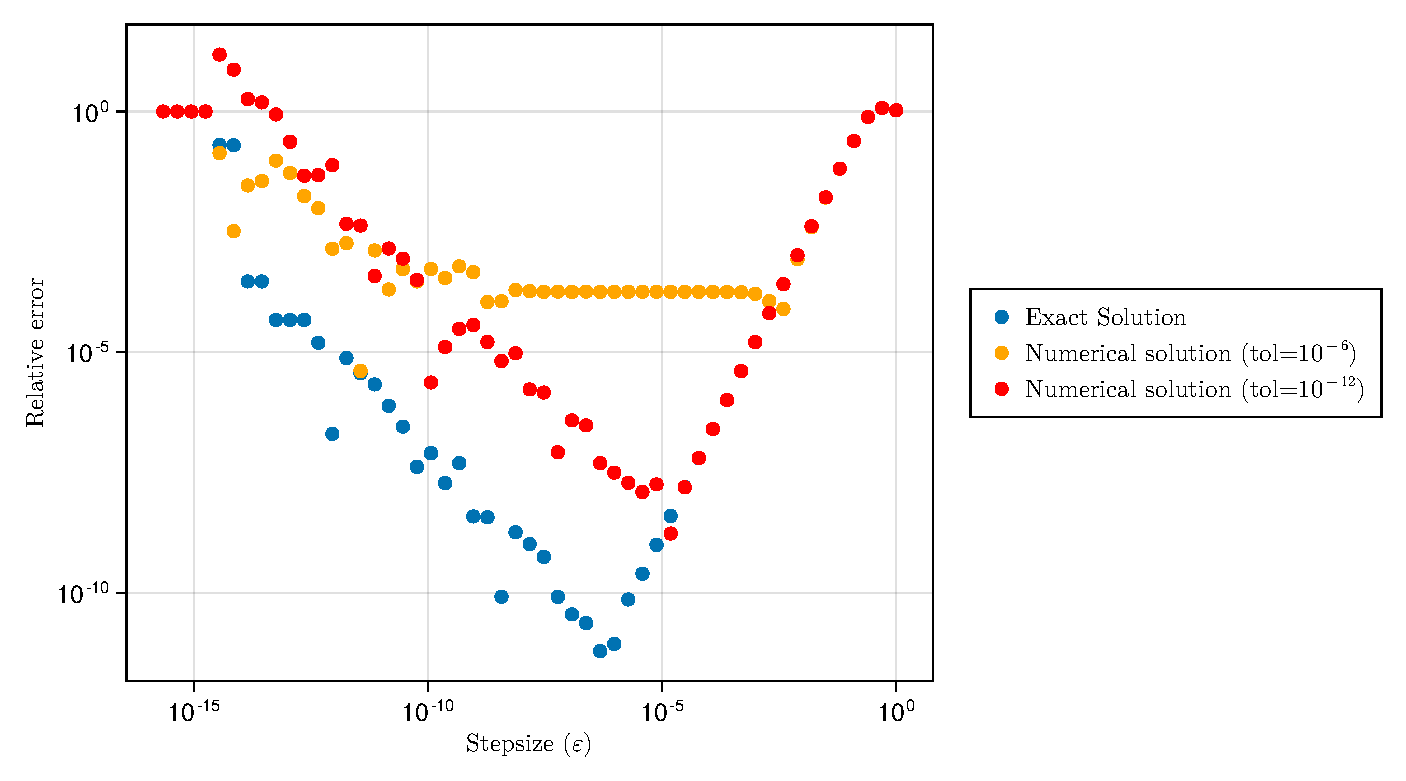
\includegraphics[width=0.85\textwidth]{../code/finite_differences/finite_difference_derivative.pdf}
    \caption{Absolute relative error when computing the gradient of the function $u(t) = \sin (\omega t)/\omega$ with respect to $\omega$ at $t=10.0$ as a function of the stepsize $\varepsilon$. Here, $u(t)$ corresponds to the solution of the differential equation $u'' + \omega^2 u = 0$ with initial condition $u(0)=0$ and $u'(0)=1$. The blue dots correspond to the case where the relative error is computed with finite differences. The red and orange lines are for the case where $u(t)$ is numerically computed using the default Tsitouras solver \cite{Tsitouras_2011} from \texttt{OrdinaryDiffEq.jl} using different tolerances. The error when using a numerical solver is larger and it is dependent on the numerical precision of the numerical solver. }
    \label{fig:finite-diff}
\end{figure}

\subsubsection{Complex step differentiation}

% For credit: The figure in the left coicindes with the one in  \cite{fike2013multi}
% Read more carefully Martins et. al. (2001) for the computational aspects of complex step.

Complex-step differentiation does not suffer from small values of $\varepsilon$, meaning that $\varepsilon$ can be chosen arbitrarily small \cite{martins2001connection} as long as it does not reach the underflow threshold \cite{Goldberg_1991_floatingpoint} (see Figure \ref{fig:finite-diff}). 
As we mentioned in section ..., complex step differentiation has many aspects in common with finite differences and AD based on dual numbers. 
% This resemblance between the methods makes them susceptible to the same advantages and disadvantages: easiness of implementation with operator overloading; and inefficient scaling with respect to the number of variables to differentiate. 
However, the difference between the methods also makes the complex step differentiation sometimes more efficient than both finite differences and AD \cite{Lantoine_Russell_Dargent_2012}, an effect that can be counterbalanced by the number of extra unnecessary operations that complex arithmetic requires (see last column in Figure \ref{fig:complex-step-AD}) \cite{Martins_Sturdza_Alonso_2003_complex_differentiation}.
We note that many modern software already have support for complex number arithmetic, making complex step differentiation very easy to implement.

\subsubsection{Automatic differentiation}

The AD algorithms described in Section ... implement algorithmic differentiation using different methods, namely \textit{operator overloading} for AD based on dual numbers, and \textit{source code transformation} for both forward and reverse AD based on the computational graph \cite{martins2001connection}.

\paragraph{Forward AD based on dual numbers}
\label{section:software-Forward-AD}

Implementing forward AD using dual numbers is usually carried out using \textit{operator overloading} \cite{Neuenhofen_2018}. 
This means expanding the object associated to a numerical value to include the tangent and extending the definition of atomic algebraic functions. 
In Julia, this can be done by relying on multiple dispatch \cite{Julialang_2017}. 
The following example illustrates how to define a dual number and its associated binary addition and multiplication extensions. 
\begin{jllisting}
using Base: @kwdef

@kwdef struct DualNumber{F <: AbstractFloat}
    value::F
    derivative::F
end

# Binary sum
Base.:(+)(a::DualNumber, b::DualNumber) = DualNumber(value = a.value + b.value, derivative = a.derivative + b.derivative)

# Binary product 
Base.:(*)(a::DualNumber, b::DualNumber) = DualNumber(value = a.value * b.value, derivative = a.value*b.derivative + a.derivative*b.value)
\end{jllisting}
We further overload base operations for this new type to extend the definition of standard functions by simply applying the chain rule and storing the derivative in the dual variable following Equation \eqref{eq:dual-number-function}:
\begin{jllisting}
function Base.:(sin)(a::DualNumber)
    value = sin(a.value)
    derivative = a.derivative * cos(a.value)
    return DualNumber(value=value, derivative=derivative)
end
\end{jllisting}
% With all these pieces together, we are able to propagate forward the value of a single-valued derivative through a series of algebraic operations. 
In the Julia ecosystem, \texttt{ForwardDiff.jl} implements forward mode AD with multidimensional dual numbers \cite{RevelsLubinPapamarkou2016}. 

Implementations of forward AD using dual numbers and computational graphs require a number of operations that increases with the number of variables to differentiate, since each computed quantity is accompanied by the corresponding gradient calculations \cite{Griewank_1989}. 
This consideration also applies to the other forward methods, including finite differences and complex-step differentiation, which makes forward models prone to the curse of dimensionality with respect to the number of parameters considered.

% If well forward AD is implemented independently of the differential equation and numerical solver, the careless combination of both can lead to disastrous numerical errors. 
Although AD is always algorithmically correct, when combined with a numerical solver \textit{AD can be numerically incorrect} and result in wrong gradient calculations. 
% Contrary to common folk, AD is not always \textit{numerically} correct and can lead to wrong gradients. 
To illustrate this point, consider the following example of a simple system of ODEs
\begin{equation}
\begin{cases}
 \frac{du_1}{dt} = a u_1 - u_1 u_2 & \quad u_1(0) = 1  \\ 
 \frac{du_2}{dt} = - a u_2 + u_1 u_2 & \quad u_2(0) = 1
\end{cases}
\end{equation}
with $a$ the parameter with respect to which we want to differentiate. 
In the simple case of $a=1$, the solutions of the ODE are constant functions $u_1(t) \equiv u_2(t) \equiv 1$. 
As explained in Appendix \ref{appendix:dual-number-solver}, traditional adaptive stepsize solvers used for just solving ODEs are designed to control for numerical errors in the ODE solution but not in its sensitivities when coupled with an internal AD method. 
This leads to wrong gradient calculations that propagate through the numerical solver without further warning. 

\paragraph{Forward AD based on computational graph}

Forward algorithmic 

\paragraph{Reverse AD based on computational graph}
\label{sec:software-reverse-AD}

In contrast to finite differences, forward AD, and complex-step differentiation, reverse AD is the only of this family of methods that propagates the gradient in backwards mode by relying on analytical derivatives of primitive functions, which in Julia are available via \texttt{ChainRules.jl}.
Since this requires the evaluation intermediate variables, reverse AD requires a more delicate protocol of how to store intermediate variables in memory and make them accessible during the backwards pass. 

Backwards AD can be implemented via \textit{pullback} functions \cite{Innes_2018}, a method also known as \textit{continuation-passing style} \cite{Wang_Zheng_Decker_Wu_Essertel_Rompf_2019}.
In the backward step, this executes a series of function calls, one for each elementary operation.
If one of the nodes in the graph $w$ is the output of an operation involving the nodes $v_1, \ldots, v_m$, where $v_i \rightarrow w$ are all nodes in the graph, then the pullback $\bar v_1, \ldots, \bar v_m = \mathcal B_w(\bar w)$ is a function that accepts gradients with respect to $w$ (defined as $\bar w$) and returns gradients with respect to each $v_i$ ($\bar v_i$) by applying the chain rule. 
Consider the example of the multiplicative operation $w = v_1 \times v_2$. Then
\begin{equation}
 \bar v_1, \bar v_2 
 \,=\,
 v_2 \times \bar w , 
 v_1 \times \bar w 
 \,=\,
 \mathcal{B}_w (\bar w),
\end{equation}
which is equivalent to using the chain rule as
\begin{equation}
 \frac{\partial \ell}{\partial v_1} = \frac{\partial}{\partial v_1}(v_1 \times v_2) \frac{\partial \ell}{\partial w}.
\end{equation}
% There are many libraries that implement reverse AD acroos programming languages \cite{Baydin_Pearlmutter_Radul_Siskind_2015}.
% In Julia, the libraries \texttt{ReverseDiff.jl} and \texttt{Zygote.jl} use pullbacks to compute gradients \cite{Innes_2018}. 
% When gradients are being computed with less than $\sim 100$ parameters, the former is faster (see documentation).

% \subsubsection{Further remarks}

A crucial distinction between AD implementations based on computational graphs is between static and dynamical methods\cite{Baydin_Pearlmutter_Radul_Siskind_2015}. 
In the case of a static implementations, the computational graph is constructed before any code is executed, which are encoded and optimized for performance within the graph language. 
For static structures such as neural networks, this is ideal \cite{abadi-tensorflow}. 
However, two major drawbacks of static methods are composability with existing code, including support of custom types, and adaptive control flow, which is a common feature of numerical solvers. 
These issues are addressed in reverse AD implementations using \textit{tracing}, where the program structure is transformed into a list of pullback functions that built the graph dynamically at runtime. 
Popular libraries in this category are \texttt{Tracker.jl} and \texttt{ReverseDiff.jl}.
There also exist source-to-source AD system that achive highest performance at the same time they support arbitrary control flow structure. 
These include \texttt{Zygote.jl}\cite{Innes_Zygote}, \texttt{Enzyme.jl}\cite{moses_Enzyme}, and \texttt{Difractor.jl}.
The existence of multiple AD packages lead to the development of \texttt{AbstractDifferentiation.jl} which allows to combine different methods \cite{Schäfer_Tarek_White_Rackauckas_2021}. 

% Since perturbation confusion also affects reverse mode AD, maybe is better to cover that here.

\paragraph{Checkpointing}
\label{section:checkpointing}

In opposition to forward AD, reverse AD requires to store in memory intermediate variables of the program. 
For a numerical solver, the number of memory required can be very large, involving a total of at least $\mathcal O(nk)$ terms, with $k$ the number of steps of the numerical solver. 
Checkpointing is a technique that can be used for all the backwards methods that avoids storing all the intermediate states by balancing  storing and recomputation to recover the required state exactly \cite{Griewank:2008kh}.

% Read chapter in Griewank!!!
% Margossian has a nice discussion on this topic

% To expand